\section{Treatment: does the map change what to do?}
\label{sec:treatment}

The prognosis chapter (Chapter~\ref{sec:prognosis}) showed that the map \emph{forecasts} who will do well; it
did not show that the map \emph{changes management}. Forecasting and prescribing are different verbs. A weather
service that reliably predicts rain has scientific value even if it cannot make the rain stop; what would make it
\emph{actionable} is if it told you that one umbrella works in this storm and a different umbrella works in that
one. This final chapter asks the harder, prescribing question: does a patient's position on the map
\emph{moderate} treatment response --- is there a position-by-treatment interaction at which the same drug helps
one phenotype and not another, the statistical object at which a coordinate would change what you prescribe?

The honest answer, set up carefully below, is a boundary rather than a breakthrough: on the observational
treatment-as-usual contained in these cohorts, the map does \emph{not} reliably moderate treatment response. That
boundary is worth drawing precisely, because it is \emph{earned} from a proper causal pipeline rather than assumed
from a shrug --- and because, in drawing it, the analysis also back-validates the prognosis of the previous
chapter and shows the archetypes describe real response heterogeneity even where they do not causally prescribe.

\subsection{The treatment data and the estimand}
\label{sub:m5data}
Treatment is recorded differently in each cohort, but all three records reduce to common drug-class exposures:
schizophrenia carries per-visit medication lists, depression drug-class strings, bipolar structured lifetime
med-class flags plus lithium plasma. From these the well-powered contrasts are \textbf{lithium in bipolar
disorder} (the classic maintenance question), \textbf{antipsychotic in bipolar disorder}, and
\textbf{clozapine in schizophrenia} (the treatment-resistance drug). The estimand is the effect of the treatment
on a two-year outcome --- co-primary functioning (EGF) and CGI response --- \emph{conditional on the patient's
position on the map}. The predictor side is exactly the object built across the previous chapters: the nine
copula coordinates, the durable trait axes, and the $A{=}4$ archetype simplex of Chapter~\ref{sec:strata}.

\begin{definitionbox}[Moderation versus a main effect]
A treatment \emph{main effect} asks whether a drug helps on average. \emph{Moderation} asks something sharper:
whether the size of that help \emph{depends on where the patient sits}. Statistically, moderation is the
$\text{treatment}\times\text{coordinate}$ interaction term. A non-zero interaction is what would let the map
\emph{select} treatment --- ``prescribe drug $A$ for the biological corner, drug $B$ elsewhere.'' This chapter
tests the interaction, not the main effect, because only the interaction is the actionable phenotype claim.
\end{definitionbox}

\begin{methodsbox}[Confounding by indication: overlap before effect]
Treatment here is prescribed on presentation, not randomized, so a naive interaction is confounded ---
sicker-looking patients receive different drugs, and that difference, not the drug, may drive the outcome. We
emulate a target trial per question. First a \emph{propensity model} estimates each patient's probability of
receiving the drug given their baseline profile,
$P(\text{treat}\mid\text{severity }[\text{CGI-S}+\text{error-corrected }G]+\text{DSM-5 arm}+\text{demographics}+\text{the 9 copula coordinates})$;
an \textbf{overlap gate} then checks there is common support --- enough comparable treated and untreated patients
to compare at all. The effect is estimated \emph{doubly-robustly}: one model for who gets treated (used to
re-weight the sample so the groups look alike on measured baseline factors --- stabilized
inverse-probability-of-treatment weighting) and one for the outcome (covariate adjustment), arranged so that if
\emph{either} model is right the estimate is unbiased. This runs inside the errors-in-variables outcome GLM of
Chapter~\ref{sec:prognosis}, now carrying a $\text{treat}\times\text{coordinate}$ interaction. The map is
\emph{both} a prescription confounder (it enters the propensity model) \emph{and} the moderator under test (its
interaction is the estimand); both roles are admissible. Each average effect carries an \textbf{E-value} --- how
strong an unmeasured confounder would have to be, on both treatment and outcome, to explain the effect away. A
small E-value means a fragile result.
\end{methodsbox}

A design point worth stating plainly: the interaction is tested against \emph{both} encodings of the map that the
previous chapters identified as load-bearing. The durable trait axes enter through errors-in-variables (they
carry genuine measurement uncertainty), and the $A{=}4$ archetypes enter through a fixed
$\text{treat}\times\text{archetype-weight}$ interaction (archetype memberships are deterministic point values, so
errors-in-variables is inappropriate for them). The two routes are run in parallel; throughout this chapter they
\emph{agree}, which is reassuring --- the verdict is not an artifact of one representation.

\subsection{The identification gate --- can we even compare?}
\label{sub:m5ident}
Before any effect can be claimed, overlap decides what is even estimable. Recall the lesson of
Chapter~\ref{sec:prognosis}: a comparison is only as good as the comparability of the groups being compared. For
each candidate drug the propensity model is fit, the sample re-weighted, and the residual imbalance measured ---
the maximum standardized mean difference across confounders after weighting.

\begin{table}[h]\centering\small\sffamily
\caption{The overlap gate. Propensity $P(\text{treat}\mid\text{severity}+\text{DSM-5}+\text{demographics}+\text{the
9 copula coordinates})$, active-comparator primary. Overlap is common support; the post-IPTW max-SMD is the
residual confounding after weighting. The clozapine row uses the on/off contrast (its active comparator is channeled).}
\label{tab:m5overlap}
\begin{tabular}{L{5.6cm} C{2.2cm} C{2.8cm} L{3.4cm}}
\toprule
\hdr{question} & \hdr{overlap} & \hdr{max-SMD (IPTW)} & \hdr{verdict}\\
\midrule
\rowcolor{facebg} lithium-BP (vs other maintenance) & $0.997$ & $0.008$ & \textbf{estimable} (clean)\\
antipsychotic-BP (vs other maintenance) & $0.996$ & $0.079$ & estimable\\
\rowcolor{facebg} clozapine-SZ (on/off) & $0.990$ & $0.068$ & estimable (channeled)\\
\bottomrule
\end{tabular}
\end{table}

\begin{keyresult}[Lithium is cleanly identified; clozapine is channeled]
The \textbf{lithium-in-bipolar} contrast has near-perfect overlap ($0.997$) and balances to negligible residual
confounding (max-SMD $0.008$) --- it is the contrast the data can genuinely support, the one place a clean causal
read is possible. Antipsychotic-in-bipolar is also estimable after weighting. \textbf{Clozapine}, reserved by
guideline for the treatment-resistant, is \emph{channeled}: its active-comparator group is not comparable, so the
analysis falls back to an on/off sensitivity contrast rather than forcing a comparison the data cannot make. The
gate tells us where to trust an answer before we compute one.
\end{keyresult}

\subsection{The map does not reliably moderate treatment response}
\label{sub:m5moderation}
On the common-support samples, the doubly-robust interaction is computed for each estimable question and outcome.
The result is the central, honest finding of the chapter: where the data are cleanest the moderation is a
\emph{well-identified null}, and where there is a hint of moderation the data cannot confirm it
(Figure~\ref{fig:m5mod}).

\begin{figure}[h]\centering
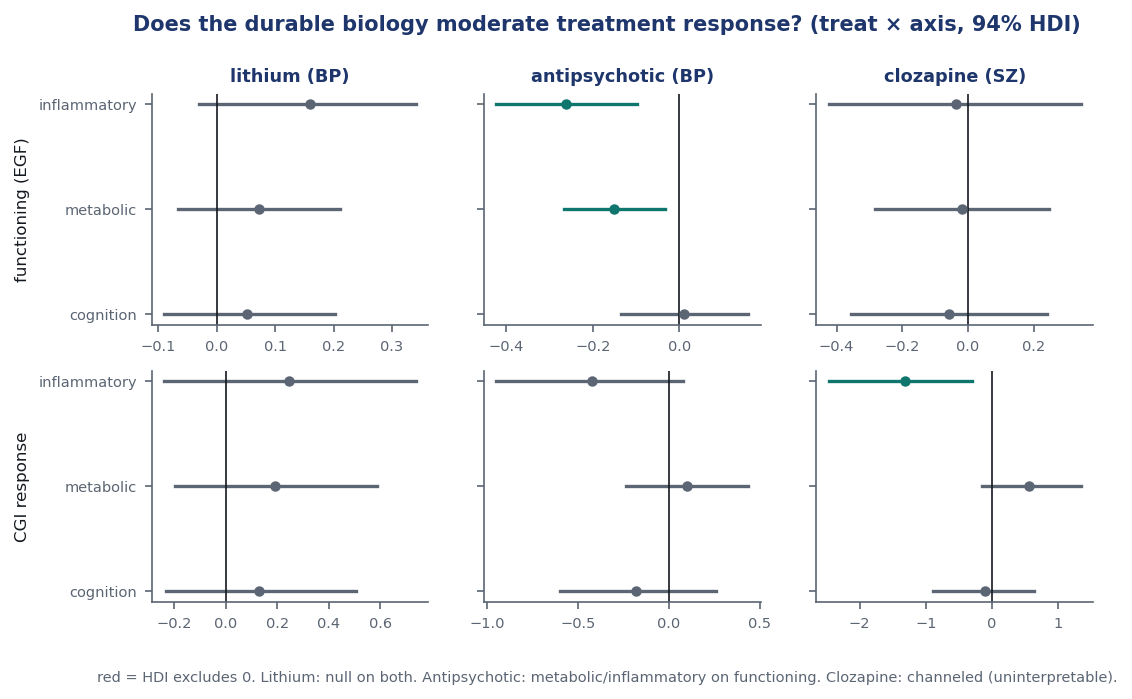
\includegraphics[width=0.96\linewidth]{figures/m5_moderation.png}
\caption{Per-drug average treatment effect (point estimate and 94\% interval) with its E-value. Lithium in
bipolar sits on zero with an E-value of $1.06$ --- a well-identified null. Antipsychotic in bipolar shows a
metabolic $\times$ functioning interaction whose interval excludes zero (inflammatory same-direction but spanning zero; ATE $-0.231$, E-value
$1.77$) but whose held-out moderation gain is weak --- suggestive but unconfirmed. Clozapine, channeled, is
non-decisive. The durable-axis and $A{=}4$-archetype encodings agree throughout.}
\label{fig:m5mod}
\end{figure}

\begin{table}[h]\centering\small\sffamily
\caption{Moderation by question and outcome: the average treatment effect with its 94\% interval, the E-value,
and the verdict. The durable and archetype representations agree (e.g.\ antipsychotic-BP functioning ATE
$-0.231$ durable vs $-0.233$ archetype; E-value $1.77$ vs $1.78$).}
\label{tab:m5moderation}
\begin{tabular}{L{4.8cm} C{3.0cm} C{1.6cm} L{4.0cm}}
\toprule
\hdr{question $\cdot$ outcome} & \hdr{ATE [94\% ETI]} & \hdr{E-value} & \hdr{verdict}\\
\midrule
\rowcolor{facebg} lithium-BP $\cdot$ functioning & $-0.003\,[-0.13,+0.12]$ & $1.06$ & \textbf{well-identified null}\\
antipsychotic-BP $\cdot$ functioning & $-0.231\,[-0.36,-0.10]$ & $1.77$ & suggestive (unconfirmed)\\
\rowcolor{facebg} antipsychotic-BP $\cdot$ CGI response & $-0.29\,[-0.66,+0.07]$ & $1.59$ & no reliable moderation\\
clozapine-SZ $\cdot$ functioning & $+0.02\,[-0.24,+0.29]$ & $1.16$ & no reliable moderation\\
\bottomrule
\end{tabular}
\end{table}

\begin{keyresult}[A well-identified null where it counts, a hypothesis where it does not]
For \textbf{lithium in bipolar} --- the best-identified contrast --- the map does \emph{not} moderate response:
the ATE sits on zero ($-0.003$, interval spanning zero) and the E-value of $1.06$ says even a trivial unmeasured
confounder would erase it. The map does not pick lithium responders. For \textbf{antipsychotic in bipolar}, the
metabolic $\times$ functioning interaction excludes zero (inflammatory same-direction but spanning zero; ATE $-0.231$, E-value $1.77$), but the
held-out moderation gain does not clear its band --- a \emph{hypothesis for prospective testing}, not a result.
Clozapine is non-decisive. The average effects are confounding-fragile throughout (E-values $1.06$--$1.78$). On
observational treatment-as-usual, the map does not reliably moderate treatment response.
\end{keyresult}

\subsection{The prognosis survives treatment adjustment}
\label{sub:m5survival}
A standing objection to the prognosis of Chapter~\ref{sec:prognosis} is that its functional forecast might be
nothing but unmodelled treatment: patients in the biological corner are medicated differently, and perhaps it is
the drugs, not the biology, that move the outcome. This is testable directly. Re-fit the functioning prognosis on
the treatment-data subset ($N=1{,}324$), once with and once without the drug-class exposures as covariates on the
same sample, and ask whether the prognostic carrier survives the adjustment.

\begin{keyresult}[M5 strengthens M4: the carrier is not a treatment proxy]
The prognostic carrier --- the low-burden archetype A1, the corner the previous chapter identified as the best
functional outcome --- \textbf{survives} treatment adjustment: its coefficient moves only $\beta=0.164\to0.156$
($4.7\%$ attenuation) and its interval still excludes zero. The map's functional forecast is therefore not merely
a relabelling of which drugs the patient was on; it holds after adjusting for the drug classes. M5 strengthens
M4 rather than undermining it (residual prescribing is bounded by the E-values above, not eliminated).
\end{keyresult}

Consistent with Chapter~\ref{sec:prognosis}, the predictive signal lives in the \emph{fuller $A{=}4$ archetype
representation} --- the biological corner read off the simplex --- and not in an isolated three-axis durable
block. On this map the durable trio alone does not survive the same adjustment (its interval includes zero);
the archetype carrier does. The lesson of the prognosis chapter repeats here: the load-bearing object is the
whole archetype geometry, with biology as one corner of it, rather than a stripped-down handful of axes.

\subsection{The map describes treatment-response heterogeneity}
\label{sub:m5heterogeneity}
Causally moderating a \emph{specific} drug and \emph{describing} response heterogeneity are different claims, and
the map can do the second even where it cannot do the first. The archetypes predict the treatment-response
endpoints --- resistance, CGI response, significant side-effects --- beyond diagnosis and severity, measured by
held-out $\Delta$ELPD (the same incremental-fit currency as Chapter~\ref{sec:prognosis}).

\begin{table}[h]\centering\small\sffamily
\caption{Response-heterogeneity description. Held-out $\Delta$ELPD of the $A{=}4$ archetypes (and of the durable
trio alone) over diagnosis $+$ severity. The archetype simplex carries a real response-stratification signal;
the durable trio alone does not.}
\label{tab:m5heterogeneity}
\begin{tabular}{L{5.4cm} C{3.4cm} C{2.6cm}}
\toprule
\hdr{endpoint} & \hdr{archetypes $\Delta$ELPD} & \hdr{durable $\Delta$ELPD}\\
\midrule
\rowcolor{facebg} treatment resistance & $+20.0\pm6.8$ & $-2.6$\\
CGI response & $+16.5\pm6.2$ & $-2.9$\\
\rowcolor{facebg} significant side-effects & $+10.4\pm5.3$ & $+2.7$\\
\bottomrule
\end{tabular}
\end{table}

The archetypes describe \emph{who} tends to be treatment-resistant, who responds, and who carries side-effect
burden, with the resistance and response gains comfortably exceeding twice their standard error. This is a
descriptive stratification signal, not a causal prescription: it says the map sees structure in how patients
respond, while the moderation analysis above says that structure is not yet a clean instruction to switch drugs
on observational data.

\subsection{What the treatment analysis establishes --- the earned boundary}
\label{sub:m5limits}

\begin{openbox}[Earned, not assumed: observational treatment-as-usual cannot show the map prescribes]
The contribution of this chapter is a boundary drawn by evidence rather than by assumption. With real treatment
data and a proper causal pipeline, the map does \emph{not} reliably moderate treatment-as-usual response: the
cleanest contrast (lithium) is a well-identified null, the antipsychotic metabolic signal is
suggestive but unconfirmed, clozapine is confounded by channeling, and the average effects are fragile to
unmeasured confounding (E-values $1.06$--$1.78$). What the analysis \emph{does} deliver is a well-identified
null where it counts, a testable hypothesis (metabolic $\times$ antipsychotic functioning), a
deployable causal method, a back-validation of the prognosis (the archetype carrier survives treatment
adjustment, $4.7\%$ attenuation), and a descriptive response-stratification signal (the archetypes predict
resistance/response/side-effects). Establishing treatment \emph{selection} --- which drug for which phenotype ---
would require the randomized or trial-arm data of a future treatment-selection study (M5b); observational
prescription data, however rich, cannot. Limits carried forward: confounding by indication is the dominant
threat; prescription, not protocol; lifetime (bipolar) versus current (schizophrenia) exposure; within-cohort
questions; channeled treatments non-estimable; held-out $\Delta$ELPD is itself unreliable on the IPTW-weighted
fits, so the moderation verdict rests on the per-axis interaction interval and the E-value, reported
transparently.
\end{openbox}
